\documentclass[a4paper]{article}

%% Language and font encodings
\usepackage[french]{babel}
\usepackage[utf8]{inputenc}
\usepackage[T1]{fontenc}

\usepackage{float}

\setlength{\parindent}{1em}
%\setlength{\parskip}{1ex plus 0.5ex minus 0.2ex}
\newcommand{\hsp}{\hspace{20pt}}
\newcommand{\HRule}{\rule{\linewidth}{0.5mm}}

\usepackage{algorithm}
\usepackage[noend]{algpseudocode}
\algnewcommand{\algorithmicand}{\textbf{ and }}
\algnewcommand{\algorithmicor}{\textbf{ or }}
\algnewcommand{\OR}{\algorithmicor}
\algnewcommand{\AND}{\algorithmicand}
\algnewcommand\algorithmicforeach{\textbf{for each}}
\algdef{S}[FOR]{ForEach}[1]{\algorithmicforeach\ #1\ \algorithmicdo}
\newcommand{\myfrac}[2]{\frac{\displaystyle {#1}}{\displaystyle {#2}}}

%% Sets page size and margins
\usepackage[a4paper,top=3cm,bottom=2cm,left=3cm,right=3cm,marginparwidth=1.75cm]{geometry}

%% Useful packages
\usepackage{amsmath}
\usepackage{amssymb}
\usepackage{graphicx}
\usepackage{subcaption}
\usepackage[colorinlistoftodos]{todonotes}
\usepackage[colorlinks=true, allcolors=blue]{hyperref}
\usepackage{graphicx}

\usepackage{enumitem}
\setitemize{label=\textbullet, font=\small}

%% equations
\usepackage{amsthm}
\usepackage[retainorgcmds]{IEEEtrantools}

%% Matlab
\usepackage[framed,numbered,autolinebreaks,useliterate]{mcode}

%% theorem and proposition
\newtheorem{prop}{Proposition}
\newtheorem*{prop*}{Proposition}
\newtheorem{thm}{Théorème}

\newenvironment{myproof}[1][\proofname]{\proof[#1]\mbox{}\\*}{\endproof}

%% references shortcuts (Arthur) 
\usepackage{suffix}
\renewcommand{\eqref}[1]{équation~\ref{#1}}
\newcommand{\algoref}[1]{algorithme~\ref{#1}}
\newcommand{\figref}[1]{figure~\ref{#1}}
\newcommand{\tabref}[1]{tableau~\ref{#1}}
\newcommand{\secref}[1]{section~\ref{#1}}
\newcommand{\probref}[1]{problème~\ref{#1}}
\newcommand{\propref}[1]{proposition~\ref{#1}}
\newcommand{\theoremref}[1]{théorème~\ref{#1}}
\newcommand{\chapref}[1]{chapitre~\ref{#1}}
\newcommand{\annexeref}[1]{annexe~\ref{#1}}
\WithSuffix\newcommand\algoref*[1]{algorithme~\ref{#1} p.~\pageref{#1}}
\WithSuffix\newcommand\figref*[1]{figure~\ref{#1} p.~\pageref{#1}}
\WithSuffix\newcommand\eqref*[1]{équation~\ref{#1} p.~\pageref{#1}}
\WithSuffix\newcommand\tabref*[1]{tableau~\ref{#1} p.~\pageref{#1}}
\WithSuffix\newcommand\secref*[1]{section~\ref{#1} p.~\pageref{#1}}
\WithSuffix\newcommand\probref*[1]{problème~\ref{#1} p.~\pageref{#1}}
\WithSuffix\newcommand\propref*[1]{proposition~\ref{#1} p.~\pageref{#1}}
\WithSuffix\newcommand\chapref*[1]{chapitre~\ref{#1} p.~\pageref{#1}}

\usepackage[backend=biber,uniquename=init,giveninits=true,
             %% "et al" pour > deux auteurs, & pour exactement 2
             uniquelist=false,maxcitenames=2,mincitenames=1,maxbibnames=99,
             isbn=false,url=false,doi=false,bibstyle=numeric
]{biblatex}
\addbibresource{references.bib}

\begin{document}

\begin{titlepage}
  \begin{center}

      \makebox[0.5\textwidth][r]{%
        
\includegraphics[width=0.33\textwidth]{images/sorbonne.png}%
    }%

      \vspace{4cm}
    % Title
    \HRule \\[0.4cm]
    { \huge \bfseries BIMA - rapport \\[0.4cm] }

      \textsc{\LARGE Reconnaissance de visages par Eigenfaces}\\[0.4cm]

    \HRule \\[0.8cm]

    % Author and supervisor
    \begin{minipage}{0.4\textwidth}
      \begin{flushleft} \large
        Kim-Anh Laura \textsc{Nguyen}\\
        \large
        Arij \textsc{Riabi}\\
        M1 DAC\\
        Promo 2018-2019 \\
      \end{flushleft}
    \end{minipage}
    \begin{minipage}{0.5\textwidth}
      \begin{flushright} \large
        \emph{Enseignant :} Arnaud \textsc{Dapogny}\\
      \end{flushright}
    \end{minipage}

      \vspace{2cm}

  \end{center}
  %\end{sffamily}
\end{titlepage}
%\maketitle

\newpage

L’objectif du TME est d’étudier les propriétés de la méthode de reconnaissance
de visages « eigenfaces ».
Nous développerons un système capable :
\begin{itemize}
    \item d’identifier un visage parmi une base de données de visages de référence
    \item de déterminer si une image contient un visage présent dans la base de données
    \item de reconnaître si une image représente un visage ou non \\
\end{itemize}

Nous disposons de la base de données de visages Yale Face Database, sur laquelle
nous appliquerons les outils développés. Cette base contient 120 images en
niveaux de gris, représentant les visages de 15 individus. Il y a 8 images par
individu, chacune correspondant à une catégorie d’images variant selon la
variation de l'expression du visage et la variation des accessoires. \\

Chaque visage sera représenté par un vecteur de caractéristiques supposées
invariantes pour une même personne, et différentes d'une personne à l'autre. Il
sera considéré comme un vecteur dans un espace ayant autant de dimensions que de
pixels dans l'image ($4096$ dans notre cas). Un ensemble de visages sera stocké
dans une matrice dont chaque colonne est un visage. En général, les images
seront contenues dans une matrice \textbf{X} de taille $d \times n$ : 

$$ \mathbf{X} = [x_1,...x_n] $$

Cette base \textbf{X} sera divisée en deux groupes : l'un sera utilisé comme jeu
d'entraînement, $\mathbf{X}^{train}$ de taille $d \times N_{train}$, l'autre
comme jeu de test, $\mathbf{X}^{test}$ de taille $d \times N_{test}$.\\

\newpage
\section*{Exercice 1 - Chargement de la base et centrage des visages}

Dans cette partie, nous calculons et affichons le "visage moyen" (ou moyenne des
visages) de la base de visages de références $\mathbf{X}^{train}$ ainsi que
quelques visages et leurs visages centrés associés. Les fonctions utilisées
(calcul du visage moyen $x_{moy}$ et centrage des visages) sont
contenues dans l'\annexeref{appendix:ex1}. Les résultats sont présentés
dans la \figref{fig:ex1}.

\begin{figure}[H]
    \centering
     
    \begin{subfigure}[c]{0.24\textwidth}
        \centering
        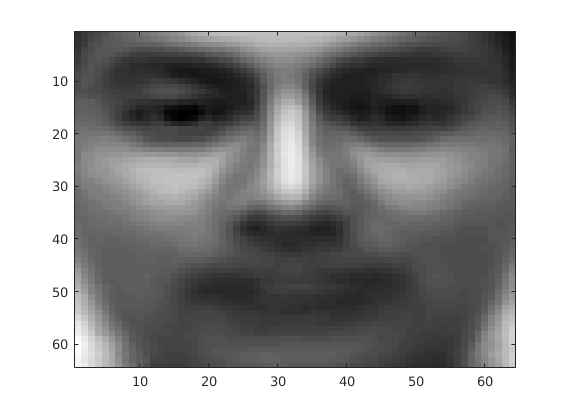
\includegraphics[width=0.8\textwidth]{images/ex1_x_centre.png}
        \caption{moyen}
        \label{subfig:ex1_x_centre}
    \end{subfigure}

    \begin{subfigure}[c]{0.24\textwidth}
        \centering
        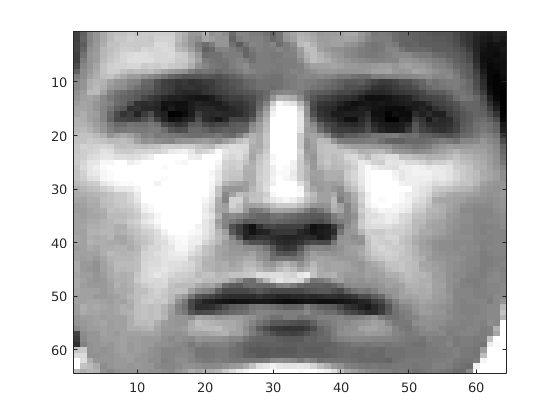
\includegraphics[width=0.8\textwidth]{images/ex1_x1.png}
        \caption{visage1}
        \label{subfig:ex1_x1}
    \end{subfigure}
    \begin{subfigure}[c]{0.24\textwidth}
        \centering
        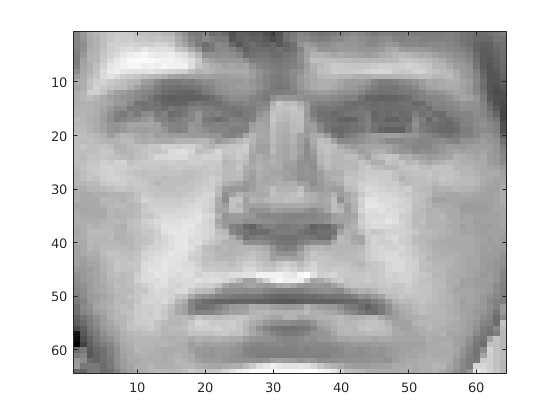
\includegraphics[width=0.8\textwidth]{images/ex1_x1c.png}
        \caption{visage1 centré}
        \label{subfig:ex1_x1c}
    \end{subfigure}
    \begin{subfigure}[c]{0.24\textwidth}
        \centering
        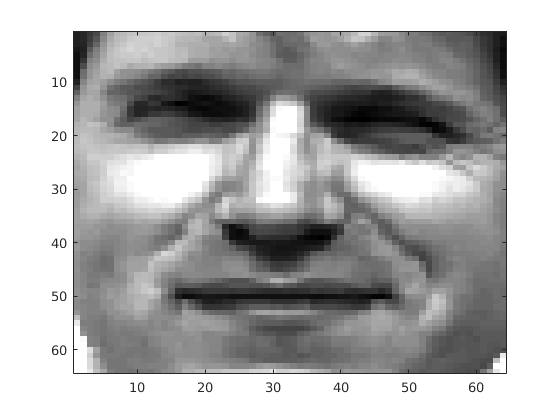
\includegraphics[width=0.8\textwidth]{images/ex1_x2.png}
        \caption{visage2}
        \label{subfig:ex1_x2}
    \end{subfigure}
    \begin{subfigure}[c]{0.24\textwidth}
        \centering
        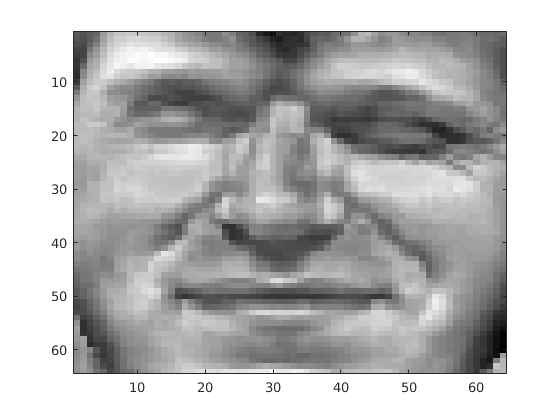
\includegraphics[width=0.8\textwidth]{images/ex1_x2c.png}
        \caption{visage2 centré}
        \label{subfig:ex1_x2c}
    \end{subfigure}

    \begin{subfigure}[c]{0.24\textwidth}
        \centering
        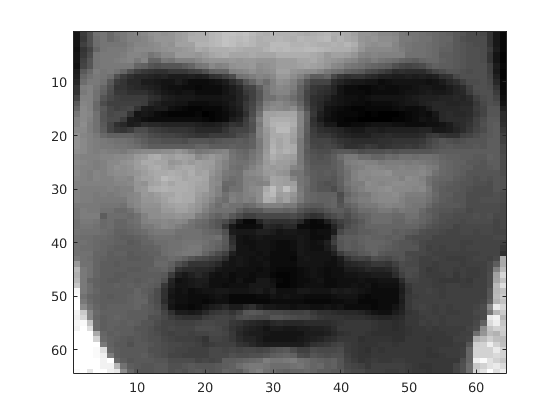
\includegraphics[width=0.8\textwidth]{images/ex1_x3.png}
        \caption{visage3}
        \label{subfig:ex1_x3}
    \end{subfigure}
    \begin{subfigure}[c]{0.24\textwidth}
        \centering
        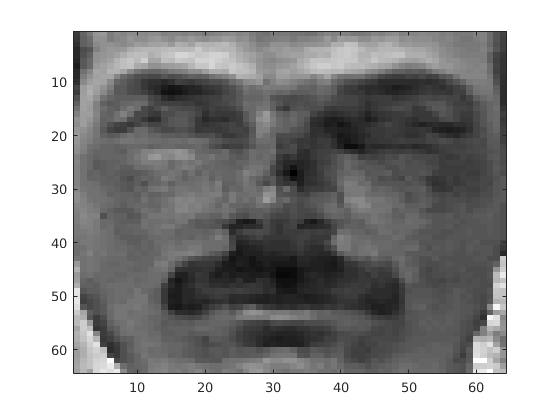
\includegraphics[width=0.8\textwidth]{images/ex1_x3c.png}
        \caption{visage3 centré}
        \label{subfig:ex1_x3c}
    \end{subfigure}
    \begin{subfigure}[c]{0.24\textwidth}
        \centering
        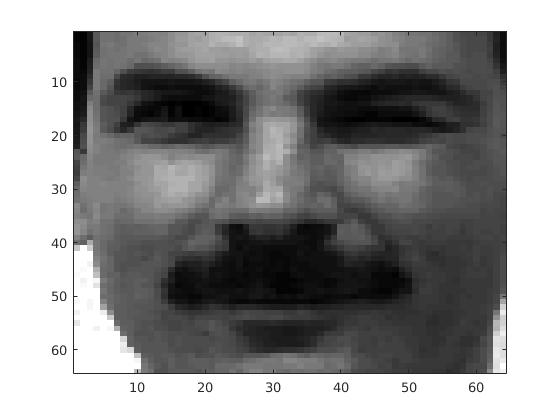
\includegraphics[width=0.8\textwidth]{images/ex1_x4.png}
        \caption{visage4}
        \label{subfig:ex1_x4}
    \end{subfigure}
    \begin{subfigure}[c]{0.24\textwidth}
        \centering
        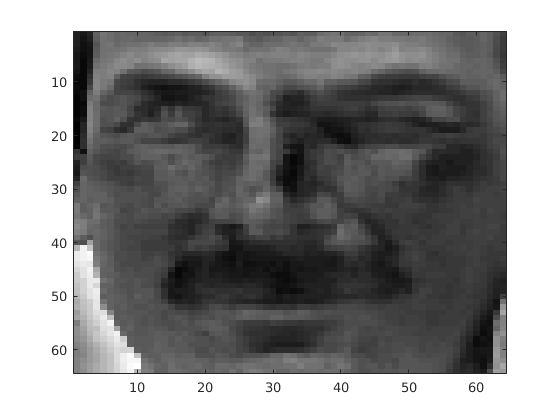
\includegraphics[width=0.8\textwidth]{images/ex1_x4c.png}
        \caption{visage4 centré}
        \label{subfig:ex1_x4c}
    \end{subfigure}

    \begin{subfigure}[c]{0.24\textwidth}
        \centering
        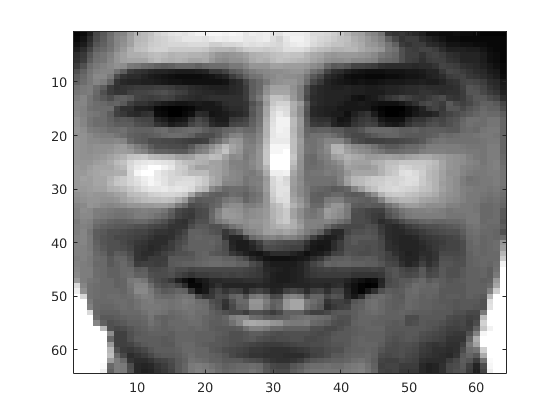
\includegraphics[width=0.8\textwidth]{images/ex1_x5.png}
        \caption{visage5}
        \label{subfig:ex1_x5}
    \end{subfigure}
    \begin{subfigure}[c]{0.24\textwidth}
        \centering
        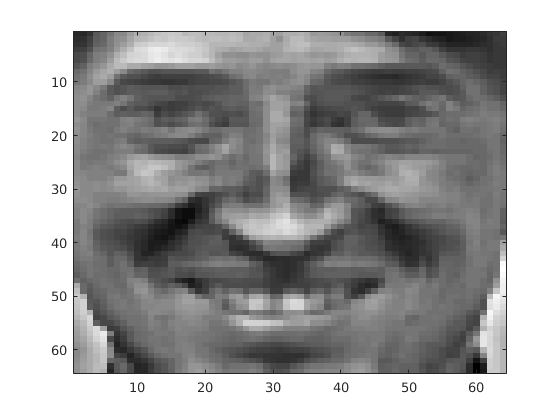
\includegraphics[width=0.8\textwidth]{images/ex1_x5c.png}
        \caption{visage5 centré}
        \label{subfig:ex1_x5c}
    \end{subfigure}
    
    \caption{Visage moyen et centrage de la base d'apprentissage} 
    \label{fig:ex1}
\end{figure}

\newpage

\section*{Exercice 2 - Calcul des Eigenfaces (ACP)}

Pour résoudre le problème de la reconnaissance de visages, nous allons utiliser
la méthode des \textit{eigenfaces}, une approche de type "image" basée sur
l'Analyse en Composantes Principales (ACP).\\

Le principe est d'extraire les caractéristiques d'un visage quelconque
$\mathit{x} \in \mathbb{R}^d$ par une méthode mathématique de réduction de
dimensionnalitée basée sur l'ACP. Les eigenfaces sont définis comme les axes
principaux obtenus en effectuant cette analyse. Il s'agit ensuite de modéliser
la différence du visage $\mathit{x}$ par rapport au visage moyen
$\mathit{x}_{moy}$ par un ensemble limité de $\mathit{K}$ images, $\mathbf{W}_K$
= $[u_1,...,\mathit{u_K}]$, appelées eigenfaces. Le visge $\mathit{x}$ est donc
exprimé comme le visage moyen auquel s'ajoute une combinaison linéaire
d'eigenfaces : 

$$ \mathit{x} = \mathit{x}_{moy} + \sum_{h=1}^{\mathit{K}} a_h u_h + \epsilon$$

où $a_h$ représente le poids de l'eigenface d'indice $h$ dans le visage
$\mathit{x}$, et $\epsilon$ représente l'erreur entre $\mathit{x}$ et son approximation
par les eigenfaces. \\

À partir de $\textbf{X}_c = [x_1 - x_{moy}, ..., x_n - x_{moy}]$, l'ensemble des
images centrées de la base d'apprentissage, nous mettons au point la fonction
\texttt{eigenfaces} (\annexeref{appendix:ex2}) qui calcule la matrice des
eigenfaces, les vecteurs propres de la matrice de covariance $\textbf{X}_c
\times \textbf{X}_c^T$, ainsi que leurs valeurs propres associées. Nous
normalisons ces dernières afin que leur somme soit égale à 100\%. \\

La \figref{fig:ex2-eigenfaces} contient le visage moyen ainsi que les 15
premières eigenfaces et leurs valeurs propres associées. \\

Les eigenfaces forment un ensemble représentant, avec un nombre de dimensions
réduit, les visages utilisés pour construire la matrice de variance co-variance. 

\begin{figure}[H]
    \centering
     
    \begin{subfigure}[c]{0.24\textwidth}
        \centering
        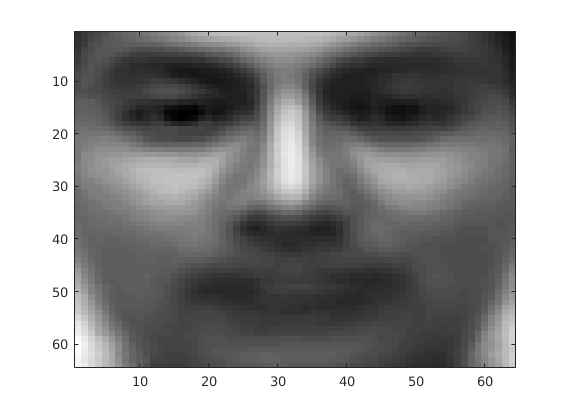
\includegraphics[width=0.65\textwidth]{images/ex1_x_centre.png}
        \caption{moyen}
        \label{subfig:ex2_x_centre}
    \end{subfigure}

    \begin{subfigure}[c]{0.24\textwidth}
        \centering
        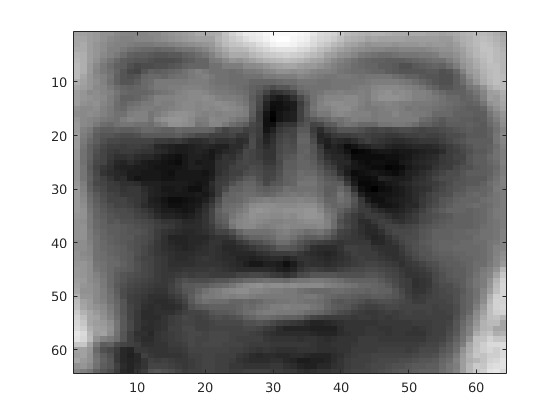
\includegraphics[width=0.65\textwidth]{images/ex2_x1.png}
        \caption{eigenface1 - 26.2631}
        \label{subfig:ex2_x1}
    \end{subfigure}
    \begin{subfigure}[c]{0.24\textwidth}
        \centering
        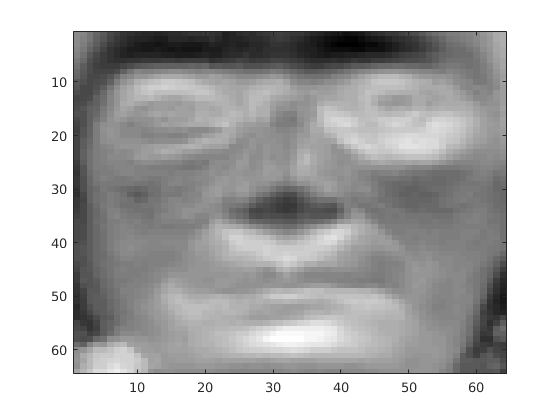
\includegraphics[width=0.65\textwidth]{images/ex2_x2.png}
        \caption{eigenface2 - 13.5651}
        \label{subfig:ex2_x2}
    \end{subfigure}
    \begin{subfigure}[c]{0.24\textwidth}
        \centering
        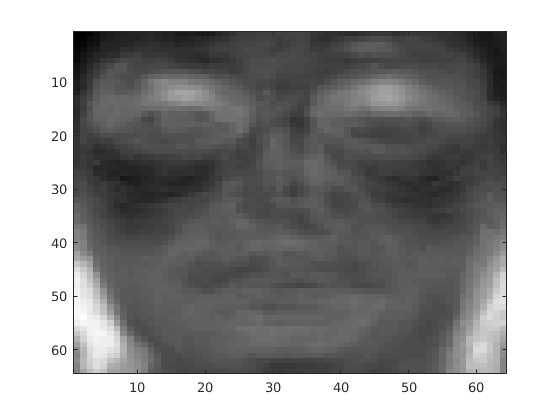
\includegraphics[width=0.65\textwidth]{images/ex2_x3.png}
        \caption{eigenface3 - 6.9953}
        \label{subfig:ex2_x3}
    \end{subfigure}
    \begin{subfigure}[c]{0.24\textwidth}
        \centering
        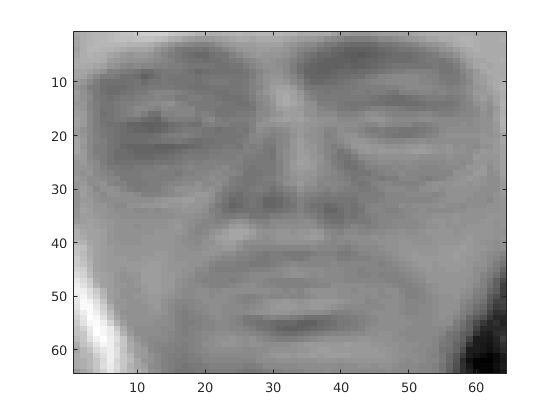
\includegraphics[width=0.65\textwidth]{images/ex2_x4.png}
        \caption{eigenface4 - 6.5426}
        \label{subfig:ex2_x4}
    \end{subfigure}

    \begin{subfigure}[c]{0.24\textwidth}
        \centering
        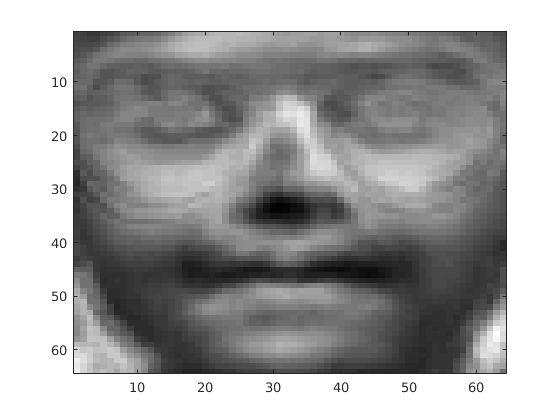
\includegraphics[width=0.65\textwidth]{images/ex2_x5.png}
        \caption{eigenface5 - 4.8841}
        \label{subfig:ex2_x5}
    \end{subfigure}
    \begin{subfigure}[c]{0.24\textwidth}
        \centering
        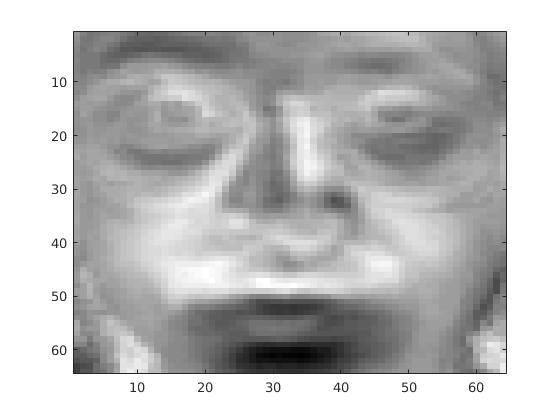
\includegraphics[width=0.65\textwidth]{images/ex2_x6.png}
        \caption{eigenface6 - 4.4261}
        \label{subfig:ex2_x6}
    \end{subfigure}
    \begin{subfigure}[c]{0.24\textwidth}
        \centering
        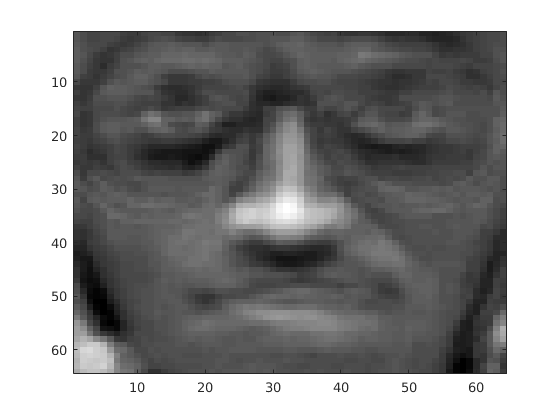
\includegraphics[width=0.65\textwidth]{images/ex2_x7.png}
        \caption{eigenface7 - 3.4697}
        \label{subfig:ex2_x7}
    \end{subfigure}
    \begin{subfigure}[c]{0.24\textwidth}
        \centering
        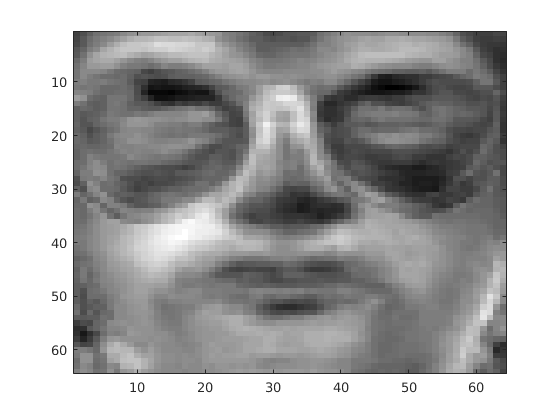
\includegraphics[width=0.65\textwidth]{images/ex2_x8.png}
        \caption{eigenface8 - 2.6741}
        \label{subfig:ex2_x8}
    \end{subfigure}

    \begin{subfigure}[c]{0.24\textwidth}
        \centering
        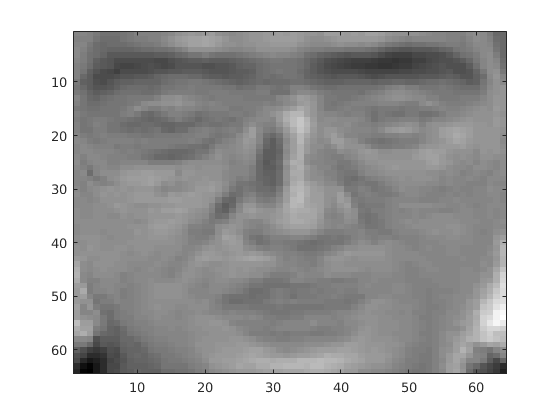
\includegraphics[width=0.65\textwidth]{images/ex2_x9.png}
        \caption{eigenface9 - 2.3953}
        \label{subfig:ex2_x9}
    \end{subfigure}
    \begin{subfigure}[c]{0.24\textwidth}
        \centering
        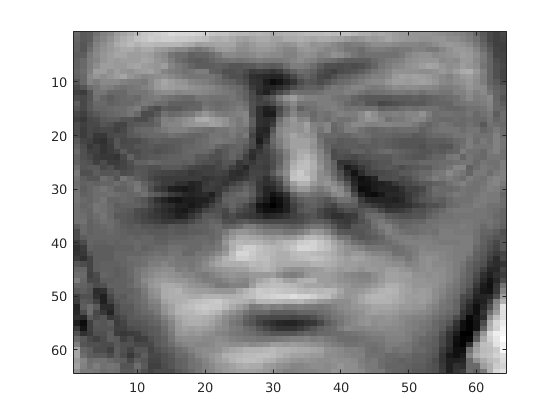
\includegraphics[width=0.65\textwidth]{images/ex2_x10.png}
        \caption{eigenface10 - 2.1801}
        \label{subfig:ex2_x10}
    \end{subfigure}
    \begin{subfigure}[c]{0.24\textwidth}
        \centering
        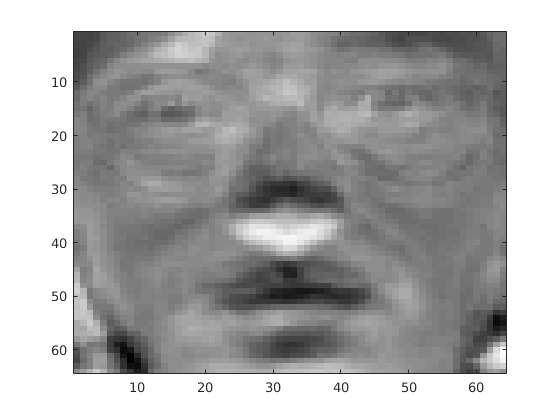
\includegraphics[width=0.65\textwidth]{images/ex2_x11.png}
        \caption{eigenface11 - 2.0269}
        \label{subfig:ex2_x11}
    \end{subfigure}
    \begin{subfigure}[c]{0.24\textwidth}
        \centering
        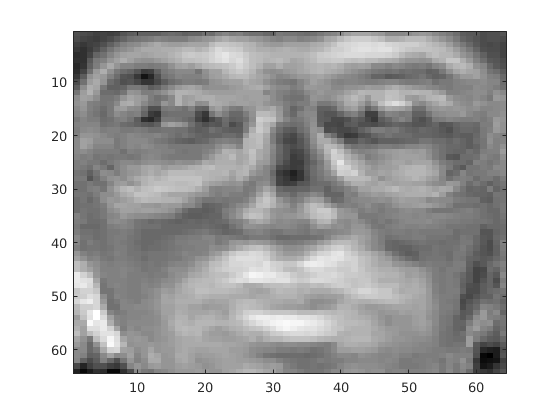
\includegraphics[width=0.65\textwidth]{images/ex2_x12.png}
        \caption{eigenface12 - 1.5541}
        \label{subfig:ex2_x12}
    \end{subfigure}

    \begin{subfigure}[c]{0.24\textwidth}
        \centering
        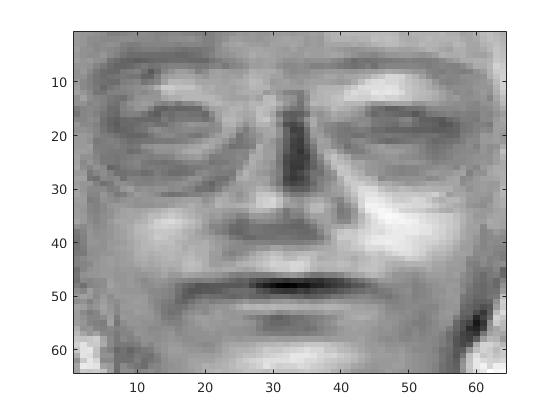
\includegraphics[width=0.65\textwidth]{images/ex2_x13.png}
        \caption{eigenface13 - 1.5020}
        \label{subfig:ex2_x13}
    \end{subfigure}
    \begin{subfigure}[c]{0.24\textwidth}
        \centering
        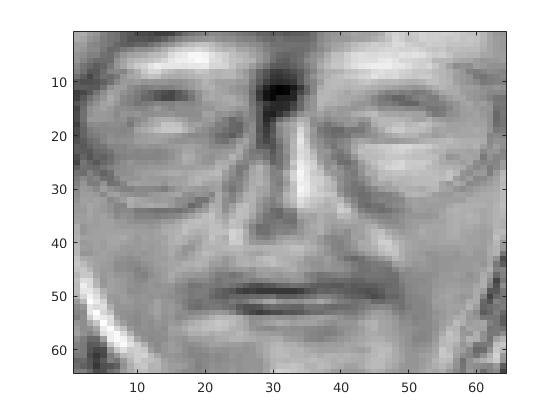
\includegraphics[width=0.65\textwidth]{images/ex2_x14.png}
        \caption{eigenface14 - 1.1538}
        \label{subfig:ex2_x14}
    \end{subfigure}
    \begin{subfigure}[c]{0.24\textwidth}
        \centering
        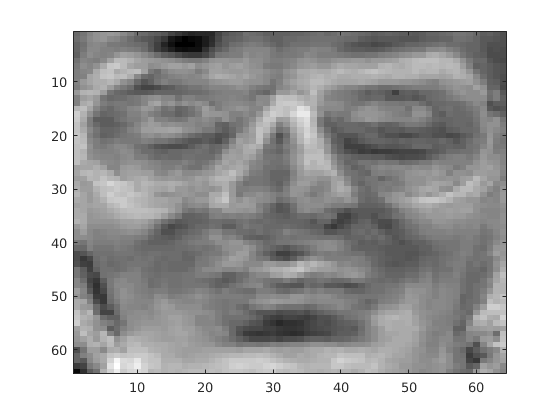
\includegraphics[width=0.65\textwidth]{images/ex2_x15.png}
        \caption{eigenface15 - 1.10.65}
        \label{subfig:ex2_x15}
    \end{subfigure}

    \caption{Visage moyen et 15 premières eigenfaces ainsi que leurs valeurs
    propres associées} 
    \label{fig:ex2-eigenfaces}
\end{figure}

Afin d'évaluer le taux de variation capturée par les $K$ premières eigenfaces,
nous traçons la courbe de la somme cumulée des valeurs propres normalisées
(\figref{fig:ex2-somme}). 

Nous constatons qu'avec $K = 30$ eigenfaces, nous capturons un taux de variation
de 90\%, ce qui permet d'avoir une "bonne" reconstruction des visages de test.

\begin{figure}[H]
    \center
    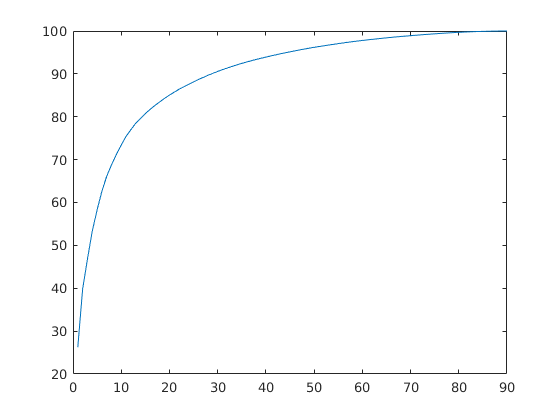
\includegraphics[width=0.6\textwidth]{images/ex2_somme.png}
    \caption{Somme cumulée des valeurs propres}
    \label{fig:ex2-somme}
\end{figure}

\newpage

\section*{Exercice 3 - Projection dans le sous-espace des visages}

Dans la suite, nous utiliserons un nombre réduit d’eigenfaces afin de modéliser
l’espace de visages représenté sous la forme de la base $\mathbf{W}_K =
[u_1,...,u_K]$ des K premiers vecteurs propres.\\

La projection d’une image $x$ dans le sous-espace des visages consiste à
soustraire le visage moyen $x_{moy}$ puis effectuer le produit scalaire de
l’image obtenue avec chaque eigenface $a_h, h \in \{1;K\}$. Ceci donne les
coordonnées de l’image test dans le sous-espace des visages, qui est de
dimension K :

$$ z = \mathbf{W}^{\top}_K \times (x - x_{moy})$$

Son image reconstruite dans l'espace d'origine $\mathbb{R}^{n}$ est :

$$ \tilde{x} = x_{moy} + \sum_{h} a_h u_h = x_{moy} + \mathbf{W}_K
\times z $$

L’erreur de reconstruction est définie comme la distance entre une image et l’image
reconstruite associée :

$$ E^{recons}(x) = || x - \tilde{x}||_2 = \sqrt{\sum_{p}(x(p) - \tilde{x}(p))^2}$$ 

Nous mettons au point une fonction \texttt{calculeProj} qui, à partir d'une
image $x$ et de l'image moyenne $x_{moy}$ de $\mathbf{X}^{train}$, calcule les
coordonnées $z$ dans le sous-espace $\mathbf{W}_K$ des visages. 

Nous écrivons également une fonction \texttt{reconstruction}, qui à partir de la
projection $z$ d’une image dans le sous-espace des visage de dimension K,
calcule les coordonnées de l’image projetée $\tilde{x}$ dans l’espace
$\mathbb{R}^n$ de départ. 

Nous implémentons aussi une fonction \texttt{erreur\_Reconstruction} qui calcule
l'erreur de reconstruction entre $x$ et $\tilde{x}$, et
\texttt{affiche\_Reconstruction}, qui affiche l'image initiale et la
reconstruction obtenue pour $K \in \{5, 10, 25, 50, 90\}$.

Ces fonctions sont contenues dans l'\annexeref{appendix:ex3}. \\

Nous utilisons ces fonctions pour projeter et reconstruire plusieurs images de
la base de référence et de test. Les figures \ref{fig:ex3-x50}, \ref{fig:ex3-x55},
et \ref{fig:ex3-x17} montrent les résultats de la
reconstruction pour, respectivement, l'image 50, 55 de $\mathbf{X}^{train}$, et
17 de $\mathbf{X}^{test}$.

\begin{figure}[H]
    \centering
     
    \begin{subfigure}[c]{0.3\textwidth}
        \centering
        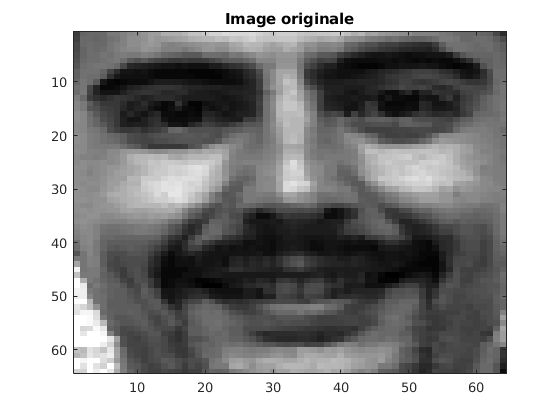
\includegraphics[width=0.8\textwidth]{images/ex3_50_originale.png}
        \caption{originale}
        \label{subfig:ex3_50_originale}
    \end{subfigure}
    \begin{subfigure}[c]{0.3\textwidth}
        \centering
        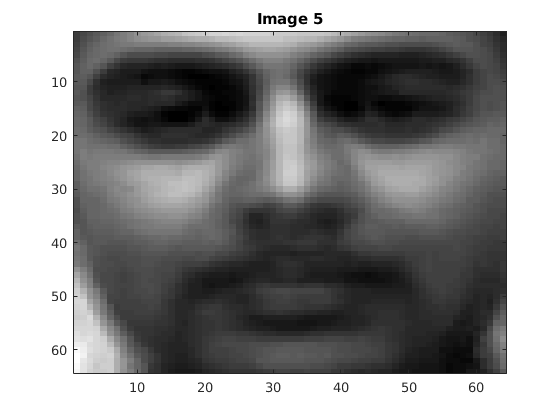
\includegraphics[width=0.8\textwidth]{images/ex3_50_5.png}
        \caption{$K=5$ - $E = 1868.6$}
        \label{subfig:ex3_50_5}
    \end{subfigure}
    \begin{subfigure}[c]{0.3\textwidth}
        \centering
        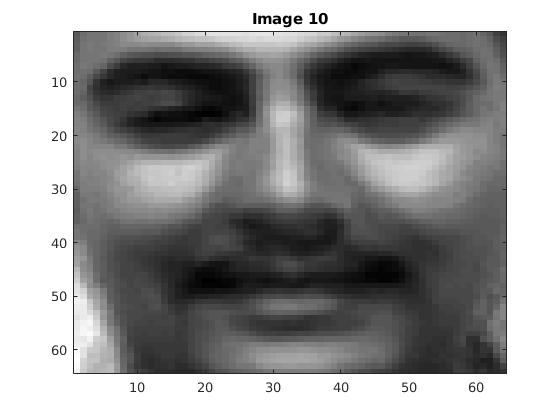
\includegraphics[width=0.8\textwidth]{images/ex3_50_10.png}
        \caption{$K=10$ - $E = 1346.9$}
        \label{subfig:ex3_50_10}
    \end{subfigure}

    \begin{subfigure}[c]{0.3\textwidth}
        \centering
        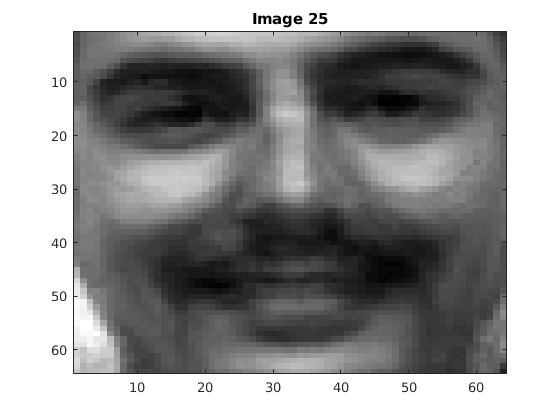
\includegraphics[width=0.8\textwidth]{images/ex3_50_25.png}
        \caption{$K=25$ - $E = 931.3975$}
        \label{subfig:ex3_50_25}
    \end{subfigure}
    \begin{subfigure}[c]{0.3\textwidth}
        \centering
        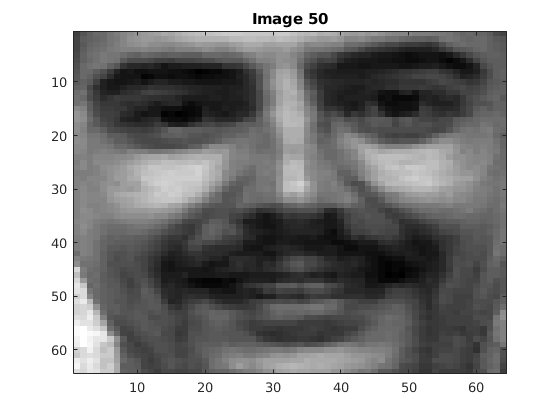
\includegraphics[width=0.8\textwidth]{images/ex3_50_50.png}
        \caption{$K=50$ - $E = 605.1090$}
        \label{subfig:ex3_50_50}
    \end{subfigure}
    \begin{subfigure}[c]{0.3\textwidth}
        \centering
        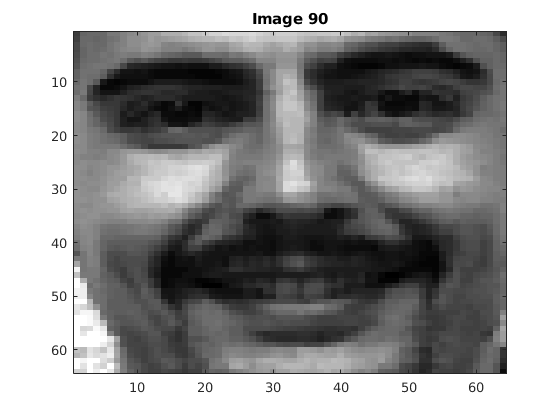
\includegraphics[width=0.8\textwidth]{images/ex3_50_90.png}
        \caption{$K=90$ - $E = 4.8975e^{-12}$}
        \label{subfig:ex3_50_90}
    \end{subfigure}

    \caption{Reconstruction de l'image 50 de la base d'apprentissage pour
    différentes valeurs de $K$} 
    \label{fig:ex3-x50}
\end{figure}

\begin{figure}[H]
    \centering
     
    \begin{subfigure}[c]{0.3\textwidth}
        \centering
        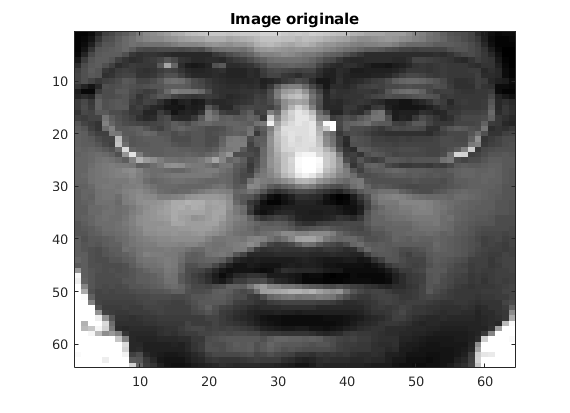
\includegraphics[width=0.8\textwidth]{images/ex3_55_originale.png}
        \caption{originale}
        \label{subfig:ex3_55_originale}
    \end{subfigure}
    \begin{subfigure}[c]{0.3\textwidth}
        \centering
        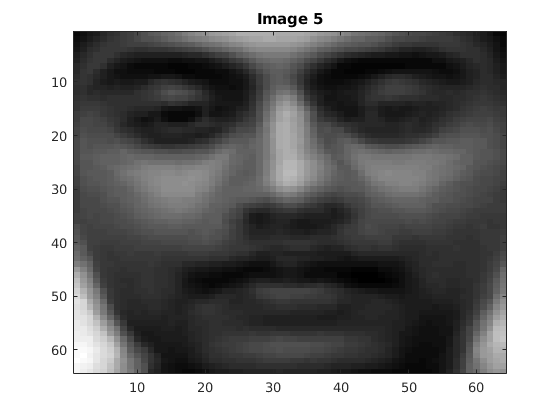
\includegraphics[width=0.8\textwidth]{images/ex3_55_5.png}
        \caption{$K=5$ - $E = 1953.7$}
        \label{subfig:ex3_55_5}
    \end{subfigure}
    \begin{subfigure}[c]{0.3\textwidth}
        \centering
        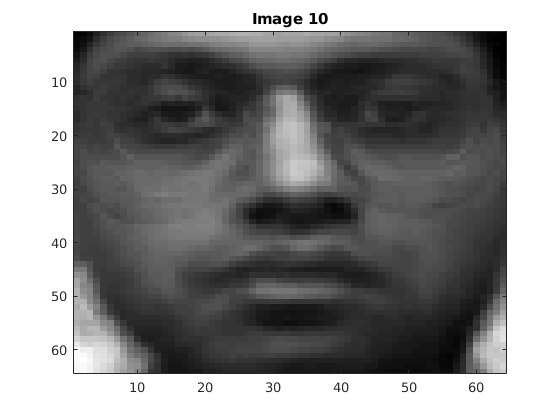
\includegraphics[width=0.8\textwidth]{images/ex3_55_10.png}
        \caption{$K=10$ - $E = 1418.2$}
        \label{subfig:ex3_55_10}
    \end{subfigure}

    \begin{subfigure}[c]{0.3\textwidth}
        \centering
        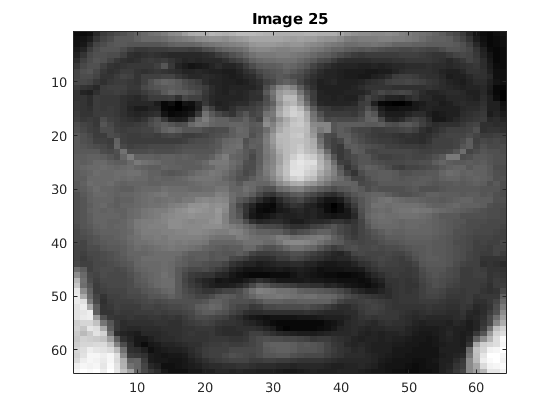
\includegraphics[width=0.8\textwidth]{images/ex3_55_25.png}
        \caption{$K=25$ - $E = 918.8$}
        \label{subfig:ex3_55_25}
    \end{subfigure}
    \begin{subfigure}[c]{0.3\textwidth}
        \centering
        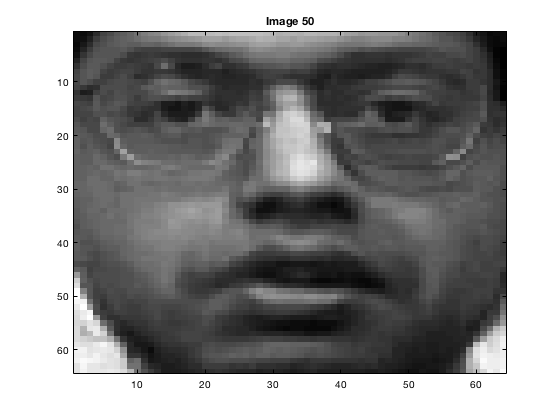
\includegraphics[width=0.8\textwidth]{images/ex3_55_50.png}
        \caption{$K=50$ - $E = 586.5$}
        \label{subfig:ex3_55_50}
    \end{subfigure}
    \begin{subfigure}[c]{0.3\textwidth}
        \centering
        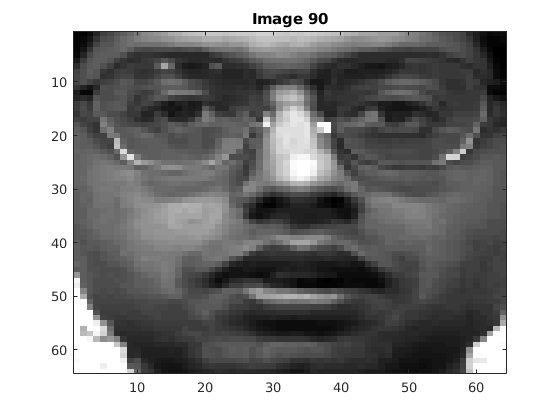
\includegraphics[width=0.8\textwidth]{images/ex3_55_90.png}
        \caption{$K=90$ - $4.4481e^{-12}$}
        \label{subfig:ex3_55_90}
    \end{subfigure}

    \caption{Reconstruction de l'image 55 de la base d'apprentissage pour
    différentes valeurs de $K$} 
    \label{fig:ex3-x55}
\end{figure}

\begin{figure}[H]
    \centering
     
    \begin{subfigure}[c]{0.3\textwidth}
        \centering
        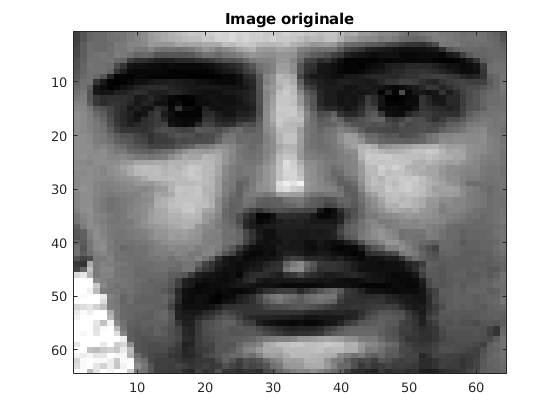
\includegraphics[width=0.8\textwidth]{images/ex3_17_originale.png}
        \caption{originale}
        \label{subfig:ex3_17_originale}
    \end{subfigure}
    \begin{subfigure}[c]{0.3\textwidth}
        \centering
        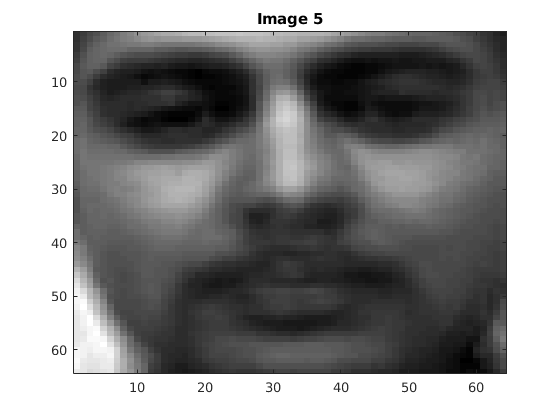
\includegraphics[width=0.8\textwidth]{images/ex3_17_5.png}
        \caption{$K=5$ - $E = 1544.9$}
        \label{subfig:ex3_17_5}
    \end{subfigure}
    \begin{subfigure}[c]{0.3\textwidth}
        \centering
        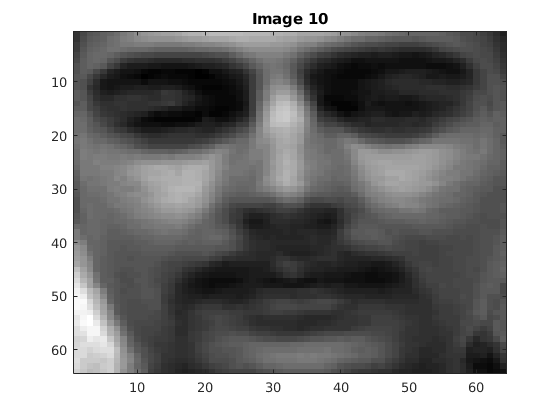
\includegraphics[width=0.8\textwidth]{images/ex3_17_10.png}
        \caption{$K=10$ - $E = 1354.4$}
        \label{subfig:ex3_17_10}
    \end{subfigure}

    \begin{subfigure}[c]{0.3\textwidth}
        \centering
        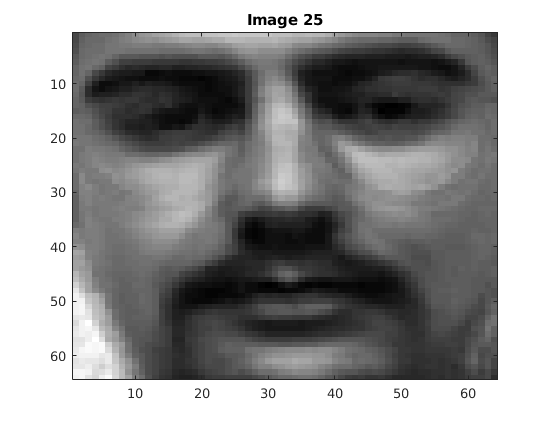
\includegraphics[width=0.8\textwidth]{images/ex3_17_25.png}
        \caption{$K=25$ - $E = 1070.5$}
        \label{subfig:ex3_17_25}
    \end{subfigure}
    \begin{subfigure}[c]{0.3\textwidth}
        \centering
        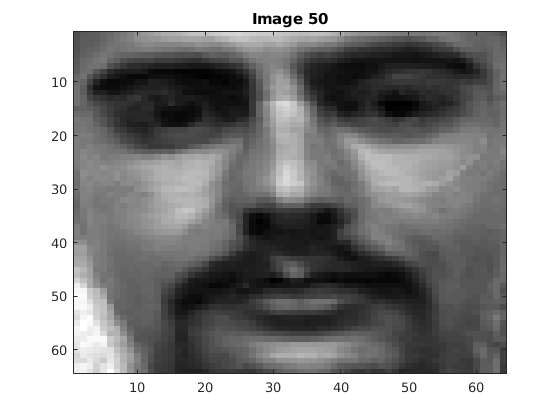
\includegraphics[width=0.8\textwidth]{images/ex3_17_50.png}
        \caption{$K=50$ - $E = 956.4$}
        \label{subfig:ex3_17_50}
    \end{subfigure}
    \begin{subfigure}[c]{0.3\textwidth}
        \centering
        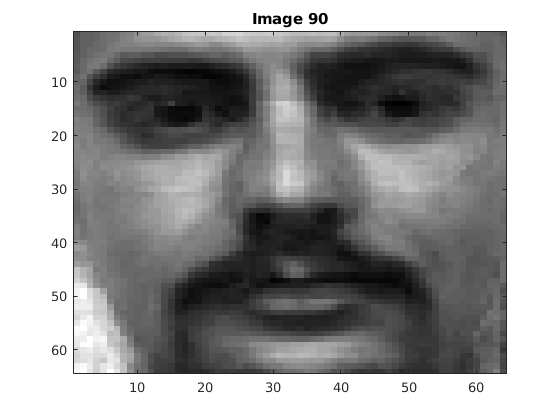
\includegraphics[width=0.8\textwidth]{images/ex3_17_90.png}
        \caption{$K=90$ - $E = 899.9$}
        \label{subfig:ex3_17_90}
    \end{subfigure}

    \caption{Reconstruction de l'image 17 de la base d'apprentissage pour
    différentes valeurs de $K$} 
    \label{fig:ex3-x17}
\end{figure}

Nous constatons sur les figures \ref{fig:ex3-x50} et \ref{fig:ex3-x55} que les
images 50 et 55 de la base d'apprentissage sont identiques à leur
reconstruction. La \figref{fig:ex3-x17} montre cependant que ce n'est pas le cas
pour l'image 17 de la base de test : alors que l'erreur de reconstruction est
quasiment nulle pour les images de $\mathbf{X}^{train}$ lorsque $K=90$
($4.4481e^{-12}$ pour l'image 55), elle est de 899.9 pour l'image de
$\mathbf{X}^{test}$.\\

Nous en concluons qu'il existe une différence en terme de reconstruction entre
les visages issus de la base d'entraînement et ceux issus de la base de test. En
effet, le sous-espace des visages dans lequel nous projetons les images est
construit à partir de la base d'apprentissage. Les images de la base de test
n'entrent, elles, pas en jeu. Les visages de $\mathbf{X}^{train}$ sont donc plus
fidèlement reconstruits que ceux de $\mathbf{X}^{test}$, et ce d'autant plus
lorsque $K$ augmente. \\

Nous traçons également l’évolution de la moyenne de l’erreur de reconstruction
des visages de test lorsque $K$ varie de 1 à $90$ (le nombre total de
eigenfaces). Le résultat est présenté dans la \figref{fig:ex3-erreur}.

\begin{figure}[H]
    \center
    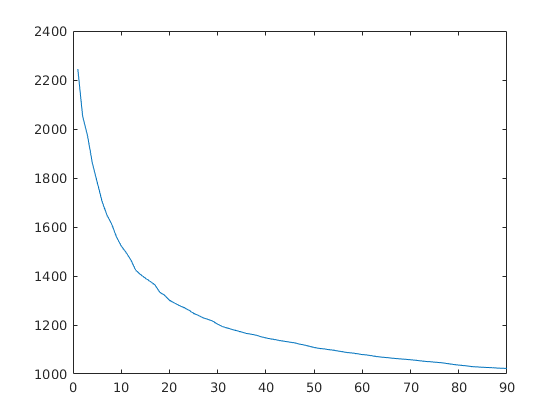
\includegraphics[width=0.6\textwidth]{images/ex3_erreur.png}
    \caption{Courbe de la moyenne de l'erreur de reconstruction des visages
    de $X_{test}$ pour $K$ variant de 1 à 90}
    \label{fig:ex3-erreur}
\end{figure}

Nous pouvons voir que la moyenne de l'erreur de reconstruction décroît
exponentiellement lorsque $K$ augmente. Ce résultat est cohérent avec la somme
cumulée calculée dans l'exercice 2 (\figref{fig:ex2-somme}).

\newpage

\section*{Exercice 4 - Reconnaissance de visage : identification}

Le problème de la reconnaissance de visages est défini de la manière suivante :
étant donnée une image de visage, on souhaite déterminer l’identité de la
personne correspondante. Nous allons comparer le vecteur de caractéristiques du
visage à reconnaître avec celui de chacun des visages de la base.\\

À chaque visage de référence $\mathit{x}^{train}_k$ est associée une identité
$id^{train}_k$. Nous allons identifier un visage $\mathit{x}^{test}$ à partir
des visages de $\mathbf{X}^{train}$.\\

Soit $\mathit{x}^{test} \in \mathbf{X}^{test}$. La méthode de reconnaissance de
visage utilisée est la suivante : 
\begin{itemize}
    \item projection de $\mathit{x}^{test}$ dans la base des eigenfaces
        $\{a_h\}_{h=1,...,K}$ 

        $$ \mathit{z^{test}} = \mathbf{W}^{\top}_K \times (\mathit{x}^{test} -
        \mathit{x}_{moy})$$
    \item calcul de la distance entre $\mathit{z}^{test}$ et la projection
        $\mathit{z}^{train}_k$ de chaque image de référence
        $\mathit{x}^{train}_k$ dans le sous-espace des visages 

        $$ E_k(\mathit{x}) = || \mathit{z}^{test} - \mathit{z}^{train}_k||_2$$
    \item détermination du visage de référence $\mathit{x}^{train}_k$ le plus
        proche du visage $\mathit{x}^{test}$. Son identifiant $id^{train}(k)$ permet
        alors la reconnaissance du visage test.\\
\end{itemize}

Il est plus intéressant de calculer la distance $E_k(\mathit{x}^{test})$ dans le
sous-espace des visages plutôt que dans l'espace de départ car ce dernier est de
trop grande dimension (autant de dimensions que de pixels dans l'image). Un
classifieur appris sur cet espace est donc trop sensible au bruit. De plus,
utiliser la base des eigenfaces diminue la complexité du problème car seules les
dimensions les plus pertinentes sont conservées. \\

Nous mettons au point une fonction \texttt{calculMatDist}
(\annexeref{appendix:ex4}) qui, à partir de l'ensemble $\mathbf{X}^{train}_c$
des images centrées d'apprentissage, de l'ensemble $\mathbf{X}^{test}_c$ des
images centrées de test, des eigenfaces $\mathbf{W}$ et de leur nombre conservé
$\mathit{K}$, calcule $D$, la matrice de distance entre les visages de test et
de référence. \\

À partir de cette matrice, nous écrivons une fonction \texttt{identification}
(\annexeref{appendix:ex4}) qui calcule le vecteur
$\hat{id}^{test}$ donnant l'indice du visage de référence le plus proche de
chaque visage de test.\\

Nous calculons maintenant, pour $K=30$, le taux d'identification en comparant
$\hat{id}^{test}$ aux labels $id^{test}$. Il est de $90\%$. 

Nous faisons ensuite varier $K$ de 1 à 90 (le nombre total de valeurs propres de
$\mathbf{W}$) puis traçons la courbe du ratio de visages reconnus en fonction de
$K$ (\figref{fig:ex4-acc}).\\

\begin{figure}[H]
    \center
    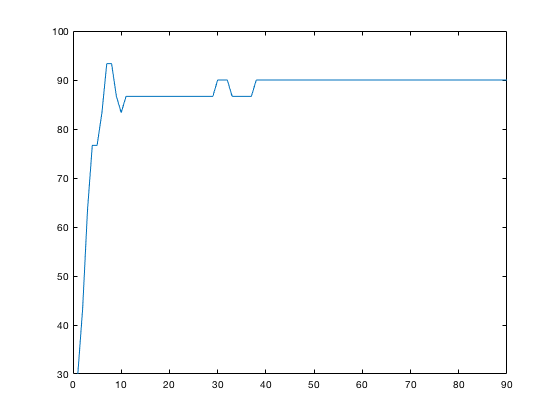
\includegraphics[width=0.6\textwidth]{images/ex4_accuracy.png}
    \caption{Taux de visages de $X_{test}$ reconnus en fonction de
    $K$}
    \label{fig:ex4-acc}
\end{figure}

La \figref{fig:ex4-acc} présente l'évolution du taux d'identification des
visages de $\mathbf{X}^{test}$ en fonction du nombre de dimensions conservées
$K$. Nous observons que, pour $K=1$ à $K=40$, le nombre de visages reconnus
augmente, puis stagne lorsque $K$ dépasse $30$ (l'allure non strictement
croissante de la courbe est justifiée par le peu de visages que contient
$\mathbf{X}^{test}$). Cela permet de montrer expérimentalement que, jusqu'à une
certaine valeur, plus le nombre de dimensions $K$ utilisées pour modéliser
l'espace de visages est grand, plus notre système est performant. Cependant, à
partir d'un certain $K$, le taux d'identification n'augmente plus et reste
constant. Cela s'explique par le fait que, les visages tests n'ayant pas servi à
l'apprentissage du modèle, ce dernier aura toujours une marge d'erreur. Pour
avoir une bonne reconnaissance et un temps de calcul faible, on peut prendre
$K=40$.\\ 

Pour $K=30$, nous calculons pour chaque visage de $\mathbf{X}^{train}$ sa
distance dans le sous-espace par rapport à l’ensemble des visages de
$\mathbf{X}^{train}$. Nous visualisons dans la \figref{subfig:ex4-bonus5mat} le
résultat sous la forme d'une image de matrice. 

Nous remarquons que la diagonale de cette matrice ne contient que des zéros. En
effet, chaque élément de cette diagonale correspond à la distance $||\mathit{z}
- \mathit{z}'||_2$ entre deux visages $x$ et $x'$ avec $x = x'$. Or, $\mathit{z}
= \mathbf{W}^{\top}_K \times (\mathit{x} - \mathit{x}_{moy}) =
\mathbf{W}^{\top}_K \times (\mathit{x'} - \mathit{x}_{moy}) = \mathit{z'}$. D'où
$||\mathit{z} - \mathit{z}'||_2 = 0$.\\

Nous traçons également l'évolution du taux de visages de référence reconnus en
fonction de $K$ (\figref{subfig:ex4-bonus5acc}), ainsi que l'évolution de ce
même taux en fonction de $K$ mais sans prendre en compte la diagonale de $D$,
i.e., les distances entre images identiques (\figref{subfig:ex4-bonus5acc2}).

Nous constatons que le premier taux d'identification est de 100\% pour toute
valeur de $K$, mais que le second varie de 30\% pour $K=1$ à plus de 90\% pour
$K=90$. En effet, en conservant cette diagonale, chaque visage de
$\mathbf{X}^{train}$ a une distance minimale avec elle-même et est donc affectée
à son propre identifiant, d'où un taux d'identification de 100\%. En supprimant
cette diagonale, on ne considère plus les distances entre images identiques et
le taux d'identification est donc plus faible (mais toujours légèrement meilleur
que pour les images de test).\\

\begin{figure}[H]
    \centering

    \begin{subfigure}[c]{0.6\textwidth}
        \centering
        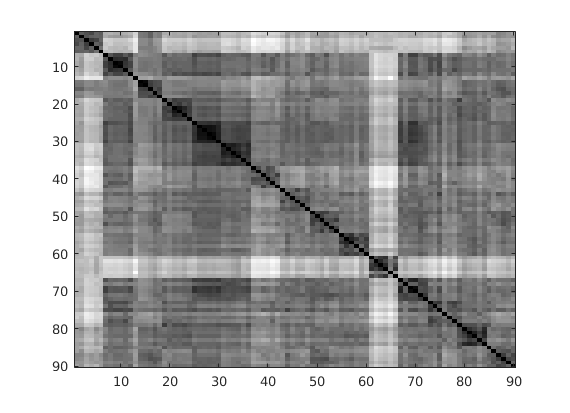
\includegraphics[width=\textwidth]{images/ex4_bonus5mat.png}
        \caption{Matrice des distances entre chaque image de $\mathbf{X}^{train}$
        dans le sous-espace des visages}
        \label{subfig:ex4-bonus5mat}
    \end{subfigure}

    \begin{subfigure}[c]{0.46\textwidth}
        \centering
        \includegraphics[width=\textwidth]{images/ex4_bonus5acc.png}
        \caption{Taux de visages de $X_{train}$ reconnus en fonction de
        $K$}
        \label{subfig:ex4-bonus5acc}
    \end{subfigure}
    \begin{subfigure}[c]{0.46\textwidth}
        \centering
        \includegraphics[width=\textwidth]{images/ex4_bonus5acc2.png}
        \caption{Taux de visages de $X_{train}$ reconnus en fonction de
        $K$, sans tenir compte de la diagonale de $D$}
        \label{subfig:ex4-bonus5acc2}
    \end{subfigure}

\end{figure}

Nous calculons également les distances minimales et maximales entre deux visages
appartenant à la même classe (même personne), et deux visages de classes
différentes. Les résultats sont présentés dans le \tabref{tab:ex4-bonus6}. Nous
constatons que les distances minimale et maximale entre deux images
correspondant au même visage sont plus petites que celles entre deux visages de
personnes différentes : notre modèle tient donc de la similitude entre images de
même classe.

\begin{table}
\centering
\resizebox{0.6\textwidth}{!}{
\begin{tabular}{|*{3}{c|}}
    \hline
        & distance minimale & distance maximale \\
        \hline
        même classe  & 270.8728 & 4426.7246\\
        classes différentes & 1264.6149 & 6730.6295\\
    \hline
\end{tabular}}
\caption{Distances min et max entre deux visages de la même classe et de
    classes différentes}
\label{tab:ex4-bonus6}
\end{table}

Nous pouvons mettre en place un seuil $\theta$ pour détecter la présence d'un
visage inconnu : si la distance minimale calculée entre un visage $x$ et un
visage de référence est supérieure à la distance maximale entre deux visages de
classe différentes, alors $x$ est un visage inconnu.

\newpage

\section*{Exercice 5 - Classification visage/non-visage}

Dans cette partie, nous utiliserons l'erreur de reconstruction pour vérifier
qu'une image est bien une image de visage. Un "non-visage" sera le terme employé
pour désigner une image contenant autre chose qu'un visage. Les non-visages sont
contenus dans la matrice $\mathbf{X}^{noface}$.\\

Nous calculons l'erreur de reconstruction des images de $\mathbf{X}^{noface}$ et
$\mathbf{X}^{test}$ en fonction de $K$. Dans les deux cas, nous calculons la
moyenne de ces erreurs, ainsi que l'erreur minimum pour les non-visages, et
l'erreur maximum pour les visages. Les courbes associées sont présentées
dans la \figref{fig:ex5-err}.

Nous constatons sur la \figref{subfig:ex5_err_mean} que les deux courbes
d'erreur décroissent de la même manière en fonction de $K$. Cependant,l'erreur
moyenne de reconstruction $E_{noface}$ des images de non-visages est
significativement supérieure à l'erreur moyenne $E_{test}$ de reconstruction des
visages ($E_{noface} - E_{test} \approx 3000$). 

Sur la \figref{subfig:ex5_min-noface_max-face}, nous observons que l'erreur de
reconstruction maximale pour une image de test est, jusqu'à $K=60$, toujours
supérieure à l'erreur de reconstruction minimale pour une image de non-visage.\\

\begin{figure}[H]
    \centering
     
    \begin{subfigure}[c]{0.6\textwidth}
        \centering
        \includegraphics[width=\textwidth]{images/ex5_err_mean_noface_test.png}
        \caption{Erreur de reconstruction moyenne}
        \label{subfig:ex5_err_mean}
    \end{subfigure}

    \begin{subfigure}[c]{0.6\textwidth}
        \centering
        \includegraphics[width=\textwidth]{images/ex5_err_min-noface_max-test}
        \caption{Erreur de reconstruction minimale pour les non-visages et
        maximale pour les visages de test}
        \label{subfig:ex5_min-noface_max-face}
    \end{subfigure}
    
    \caption{Erreur de reconstruction des images de la base de non-visages et
    des images de visages test en fonction de $K$} 
    \label{fig:ex5-err}
\end{figure}

\begin{figure}[H]
    \centering
     
    \begin{subfigure}[c]{0.24\textwidth}
        \centering
        \includegraphics[width=0.8\textwidth]{images/ex5_face1.png}
    \end{subfigure}
    \begin{subfigure}[c]{0.24\textwidth}
        \centering
        \includegraphics[width=0.8\textwidth]{images/ex5_face2.png}
    \end{subfigure}    
    \begin{subfigure}[c]{0.24\textwidth}
        \centering
        \includegraphics[width=0.8\textwidth]{images/ex5_face3.png}
    \end{subfigure}    
    \begin{subfigure}[c]{0.24\textwidth}
        \centering
        \includegraphics[width=0.8\textwidth]{images/ex5_face4.png}
    \end{subfigure}    

    \begin{subfigure}[c]{0.24\textwidth}
        \centering
        \includegraphics[width=0.8\textwidth]{images/ex5_face5.png}
    \end{subfigure}    
    \begin{subfigure}[c]{0.24\textwidth}
        \centering
        \includegraphics[width=0.8\textwidth]{images/ex5_face6.png}
    \end{subfigure}    
    \begin{subfigure}[c]{0.24\textwidth}
        \centering
        \includegraphics[width=0.8\textwidth]{images/ex5_face7.png}
    \end{subfigure}    
    \begin{subfigure}[c]{0.24\textwidth}
        \centering
        \includegraphics[width=0.8\textwidth]{images/ex5_face8.png}
    \end{subfigure}    

    \begin{subfigure}[c]{0.24\textwidth}
        \centering
        \includegraphics[width=0.8\textwidth]{images/ex5_face9.png}
    \end{subfigure}    
    \begin{subfigure}[c]{0.24\textwidth}
        \centering
        \includegraphics[width=0.8\textwidth]{images/ex5_face10.png}
    \end{subfigure}    

    \caption{Reconstruction de 10 images de la base $\mathbf{X}^{test}$} 
    \label{fig:ex5-rec-faces}
\end{figure}

\begin{figure}[H]
    \centering
     
    \begin{subfigure}[c]{0.24\textwidth}
        \centering
        \includegraphics[width=0.8\textwidth]{images/ex5_noface1.png}
    \end{subfigure}
    \begin{subfigure}[c]{0.24\textwidth}
        \centering
        \includegraphics[width=0.8\textwidth]{images/ex5_noface2.png}
    \end{subfigure}    
    \begin{subfigure}[c]{0.24\textwidth}
        \centering
        \includegraphics[width=0.8\textwidth]{images/ex5_noface3.png}
    \end{subfigure}    
    \begin{subfigure}[c]{0.24\textwidth}
        \centering
        \includegraphics[width=0.8\textwidth]{images/ex5_noface4.png}
    \end{subfigure}    

    \begin{subfigure}[c]{0.24\textwidth}
        \centering
        \includegraphics[width=0.8\textwidth]{images/ex5_noface5.png}
    \end{subfigure}    
    \begin{subfigure}[c]{0.24\textwidth}
        \centering
        \includegraphics[width=0.8\textwidth]{images/ex5_noface6.png}
    \end{subfigure}    
    \begin{subfigure}[c]{0.24\textwidth}
        \centering
        \includegraphics[width=0.8\textwidth]{images/ex5_noface7.png}
    \end{subfigure}    
    \begin{subfigure}[c]{0.24\textwidth}
        \centering
        \includegraphics[width=0.8\textwidth]{images/ex5_noface8.png}
    \end{subfigure}    

    \begin{subfigure}[c]{0.24\textwidth}
        \centering
        \includegraphics[width=0.8\textwidth]{images/ex5_noface9.png}
    \end{subfigure}    
    \begin{subfigure}[c]{0.24\textwidth}
        \centering
        \includegraphics[width=0.8\textwidth]{images/ex5_noface10.png}
    \end{subfigure}    

    \caption{Reconstruction de 10 images de la base $\mathbf{X}^{noface}$} 
    \label{fig:ex5-rec-nofaces}
\end{figure}

Nous constatons sur la \figref{fig:ex5-rec-nofaces} que les images reconstruites
n'ont aucune cohérence avec les images de départ. Notre modèle essaye de
reconstruire des visages alors que les images passées en entrées n'en sont pas.
Ce problème est dû au fait que la technique que nous utilisons se base sur la
projection d'images dans un sous-espace de visages, et qu'elle ne peut donc être
utilisée que pour la reconnaissance de visages.

%%%% ANNEXES %%%%
\appendix
\newpage

\section{Exercice 1 - Fonctions}
\label{appendix:ex1}

\begin{itemize}
    \item \texttt{calculMoy}
\begin{lstlisting}[frame=single]
function [Imoy]=calculMoy(I)
    Imoy=mean(I,2);
end
\end{lstlisting}

\item \texttt{calculCen}
\begin{lstlisting}[frame=single]
function [B_c]=CalculCen(B_I,moy)
    B_c=B_I-moy;
end
\end{lstlisting}
\end{itemize}


\section{Exercice 2 - Fonctions}
\label{appendix:ex2}
\begin{itemize}
    \item \texttt{eigenfaces}
\begin{lstlisting}[frame=single]
function[U,lambdas]=eigenfaces(Xc)
[U,S,V] = svd(Xc,0);
lambdas = diag(S).^2;
end
\end{lstlisting}
\end{itemize}

\section{Exercice 3 - Fonctions}
\label{appendix:ex3}

\begin{itemize}
    \item \texttt{calculeProj}
\begin{lstlisting}[frame=single]
function [z] = calculeProj(x,x_moy,K,W)
    z = W(:,1:K)' * (x - x_moy);
end
\end{lstlisting}

\item \texttt{reconstruction}

\begin{lstlisting}[frame=single]
function [x_r] = reconstruction(z,x_moy,K,W)
    x_r = x_moy + W(:,1:K) * z;
end
\end{lstlisting}

\item \texttt{erreur\_Reconstruction}

\begin{lstlisting}[frame=single]
function [Er] = erreur_Reconstruction(x_r,x)
    Er = sqrt(sum((x_r - x).^2));
end
\end{lstlisting}

\item \texttt{affiche\_Reconstruction}

\begin{lstlisting}[frame=single]
function [Er] = affiche_Reconstruction(x, x_moy, U)
    figure(1);
    colormap(gray);
    imagesc(reshape(x,[64,64]));
    
    title("Image originale");
    K_ = [5, 10, 25, 50, 90];
    Er = zeros(1,5);
    for i=1:5
        k = K_(i);
        z = calculeProj(x, x_moy, k, U);
        x_r = reconstruction(z, x_moy, k, U);
        Er(1,i) = erreur_Reconstruction(x_r, x);
        figure(k);
        colormap(gray);
        imagesc(reshape(x_r,[64,64]));
        title(strcat("Image ", int2str(k)));
    end
end

\end{lstlisting}
\end{itemize}

\section{Exercice 4 - Fonctions}
\label{appendix:ex4}

\begin{itemize}
    \item \texttt{calculMatDist}
\begin{lstlisting}[frame=single]
function [D] = calculMatDist(Xc_train, Xc_test, W, K)
    [p, n] = size(Xc_train);
    [q, m] = size(Xc_test);
    z_train =W(:,1:K)'* Xc_train;
    z_test  = W(:,1:K)'*Xc_test;
    D = zeros(n, m);
    for i=1:n
        for j=1:m
            t = (z_train(:, i) - z_test(:, j)) .^2;
            D(i, j) = sqrt(sum(t));
    
        end
    end
    D = D'; 
end
\end{lstlisting}

\item \texttt{identification}
\begin{lstlisting}[frame=single]
function [ id_test_hat ] = identification( D )
    [p, id_test_hat] = min(D'); 
end
\end{lstlisting}
\end{itemize}



\end{document}
